Go言語は完全なコマンド操作ツールセットを持つ言語です。コマンドラインでgoを実行することでそれらを確認することができます:

\begin{figure}[H]
   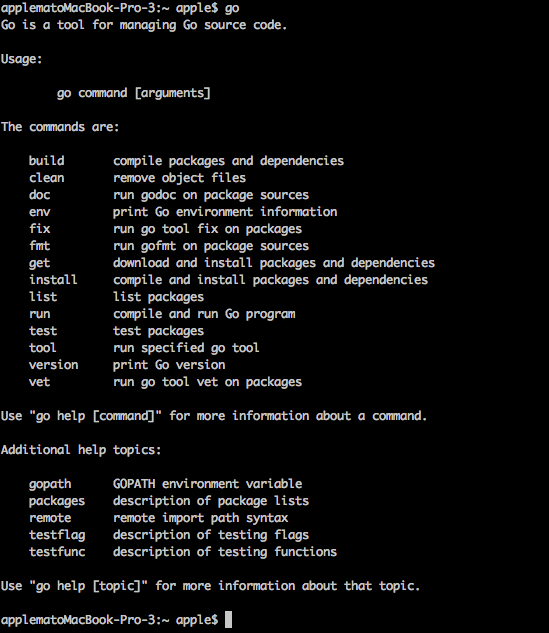
\includegraphics[width=14cm]{1.1.mac.png}
   \label{図1.3}
   \caption{Goコマンドで詳細情報を表示}
\end{figure}

これらのコマンドは我々が普段コードを書いている時に非常に役立つものです。次に普段使用するコマンドを理解していきましょう。
